\documentclass[%notes,
%handout,
usenames,dvipsnames] {beamer}
\usepackage{booktabs}
\usepackage{gensymb}
\usepackage{lmodern}
\usepackage{ragged2e}
\usepackage[spanish,mexico]{babel}
\usepackage[T1]{fontenc}
\usepackage[utf8]{inputenc}
\usepackage{textcomp}


%\usepackage{pgfpages}
%\setbeameroption{show notes on second screen}
\setbeamertemplate{navigation symbols}{}

\graphicspath{{./graphics/}}
\usecolortheme{whale}
\justifying

\definecolor{source}{HTML}{E6E6FA}
\definecolor{output}{HTML}{E6DFCF}

\setbeamertemplate{blocks}[rounded][shadow=true]
\definecolor{block}{HTML}{E6E6FA}
\definecolor{title}{HTML}{3333B3}
\setbeamercolor{block body}{bg=block}
\setbeamercolor{block title}{bg=title,fg=white}

\title{\textbf{Estadística y Probabilidad}}
\author{Alejandro Pimentel}
\date{}

%\AtBeginSection[]
%{
%  \begin{frame}
    %\frametitle{Contenido}
%    \begin{columns}[t]
%    \column{0.4\textwidth}
%    \LARGE
%    \tableofcontents[currentsection]
%    \end{columns}
%  \end{frame}
%}

\AtBeginSection[]{
  \begin{frame}
  \vfill
  \centering
  \begin{beamercolorbox}[sep=8pt,center]{title}
    \usebeamerfont{title}\insertsectionhead\par%
  \end{beamercolorbox}
  \vfill
  \end{frame}
}


\usepackage{graphicx}
\begin{document}

\frame{\titlepage}


\section{Introducción}


\frame{
\frametitle{Estadística}
\begin{block}{}
	Muchas veces nos vemos enfrentados a una masa de datos que necesita ser resumida e
interpretada. Un propósito de la estadística es proveernos de herramientas gráficas y
numéricas para esa tarea.
\end{block}
\begin{block}{}
	La estadística es el conjunto de técnicas para describir grupos de datos y para tomar decisiones en ausencia de una información completa
\end{block}
}



\frame{
\frametitle{Variables}
\begin{block}{}
	Una variables es una característica observable de un objeto, algo que se puede medir o categorizar, es aquello que se registra, los datos.
\end{block}
\begin{center}
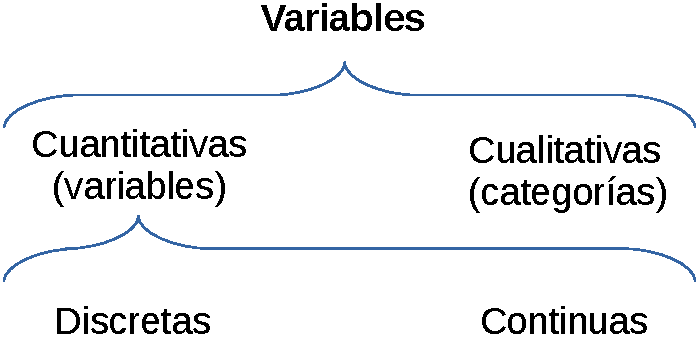
\includegraphics[width=0.8\textwidth]{variables.pdf}
\end{center}
}
\note{
Claramente es algo que puede variar, no dentro de cada objeto, sino que cada objeto puede tener un valor diferente
}



\frame{
\frametitle{Escalas}
\begin{block}{}
	La escala es la forma en la que se representa y manejar una variable. Hay diferentes tipos de escalas a considerar.
\end{block}
\begin{center}
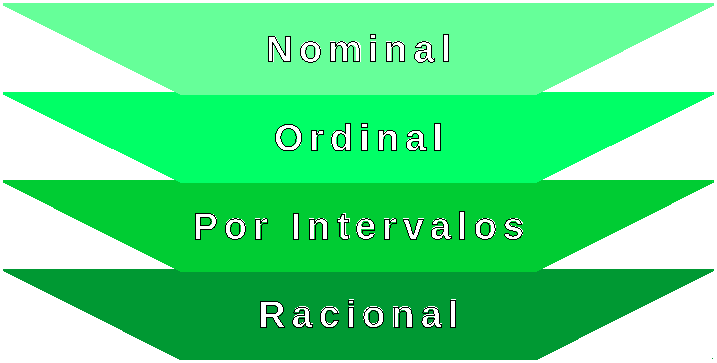
\includegraphics[width=0.6\textwidth]{escalas.pdf}
\end{center}
}


\frame{
\frametitle{Nominal}
\framesubtitle{Escalas}
\begin{block}{}
	Es una escala que se usa para atributos. Los objetos se distinguen con base en un nombre, muchas veces dado por un número o una etiqueta. Por ejemplo en el sexo de personas, se puede acordar como \textbf{H} y \textbf{M},o bien como un número. ya sea \textbf{0} o \textbf{1}.
\end{block}
\begin{center}
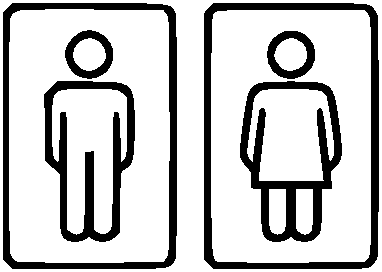
\includegraphics[width=0.5\textwidth]{h_m.pdf}
\end{center}
}



\frame{
\frametitle{Ordinal}
\framesubtitle{Escalas}
\begin{block}{}
	Esta escala refleja un \emph{ranking}. Los objetos distinguen una diferencia cualitativa  relativa de una característica que poseen.
\end{block}
\begin{center}

\includegraphics[width=\textwidth]{emojis_escala.pdf}
\end{center}
}
\note{
 Las opiniones subjetivas son un buen ejemplo de este tipo de escalas. En particular, la escala Likert es muy utilizada para medir opinión o aceptación sobre un tema.
}



\frame{
\frametitle{Por intervalos}
\framesubtitle{Escalas}
\begin{block}{}
	Cuando las diferencias entre objetos tiene sentido, tiene una medida fija. Generalmente tienen un cero, aunque este es arbitrario, como en el caso de la temperatura o las fechas.
\end{block}
\begin{center}

\includegraphics[width=0.75\textwidth]{intervalos.pdf}
\end{center}
}



\frame{
\frametitle{Racional}
\framesubtitle{Escalas}
\begin{block}{}
	Cuando no sólo las diferencias, sino también el escalamiento entre los objetos tiene sentido, la escala es racional.
\end{block}
\begin{center}

\includegraphics[width=0.8\textwidth]{racional.pdf}
\end{center}
}



\frame{
\frametitle{Escalas}
\begin{block}{}
	Hay una jerarquía en la escala presentada, al bajar la escala se pierde potencia del análisis.
\end{block}
\begin{center}
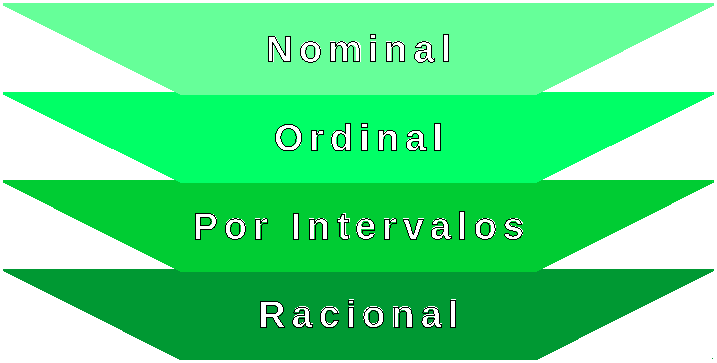
\includegraphics[width=0.6\textwidth]{escalas.pdf}
\end{center}
}
\note
{
Cabe notar que en nuestra imagen las escalas se muestran en el orden en el que fueron presentadas, es decir de la más baja a la más alta jerarquía. Al decir "{}bajar"{} la escala, nos referimos a "{}subir"{} según la imagen.
}


\end{document}
